\subsection{User Bootstrapping - Tianyuan}
\label{sec:dataop-bootstrap}
In order to bootstrap a Hydra user into the system, each Hydra user needs to obtain trust anchor, trust policies of Hydra and and get certified by the Hydra NOC

In Hydra, each user obtains the Hydra trust anchor and initial trust policies out-of-band.
After that, Hydra NOC authenticates each user on their email addresses.
This requires Hydra NOC knowing trustworthy email addresses via initial out-of-band trust relations.
We rely on the human trust relations between users and the NOC operator to realize the user authentication. 
The NOC operator maintains a list of trustworthy email addresses and configures the it to the NOC application.

Hydra user utilizes NDNCERT~\cite{} to perform the email authentication and obtains certificate from NOC.
Specifically, Hydra NOC as the NDNCERT CA does the following steps upon receiving a certificate request from a Hydra user.
It first checks the Hydra user email address membership, then verifies the email address by sending a PIN and requesting sending back in NDNCERT message.
Upon successful email membership and possession verification, Hydra NOC uses the user naming convention\ty{where's the user naming convention?} to assign the user an NDN name based on its email and certifies it.

As the final step, a Hydra user completes its security bootstrapping by obtaining and installing the issued certificate.

\subsection{Data Insertion} \label{sec:data-insert}

\subsubsection{Scenario}
Alice, a graduate student who is doing research at the Clemson's Genomics and Bioinformatics facility, has produced a pre-processed (i.e. indexed) axolotl genome that she believes is critical in understanding an axolotl's ability to regenerate tissue. She desires to publish this data in the form of a File within Hydra. To satisfy this scenario, she performs the following interactions with Hydra.


\subsubsection{User-to-Node Interaction}
\begin{figure}[!ht]
    \centering
    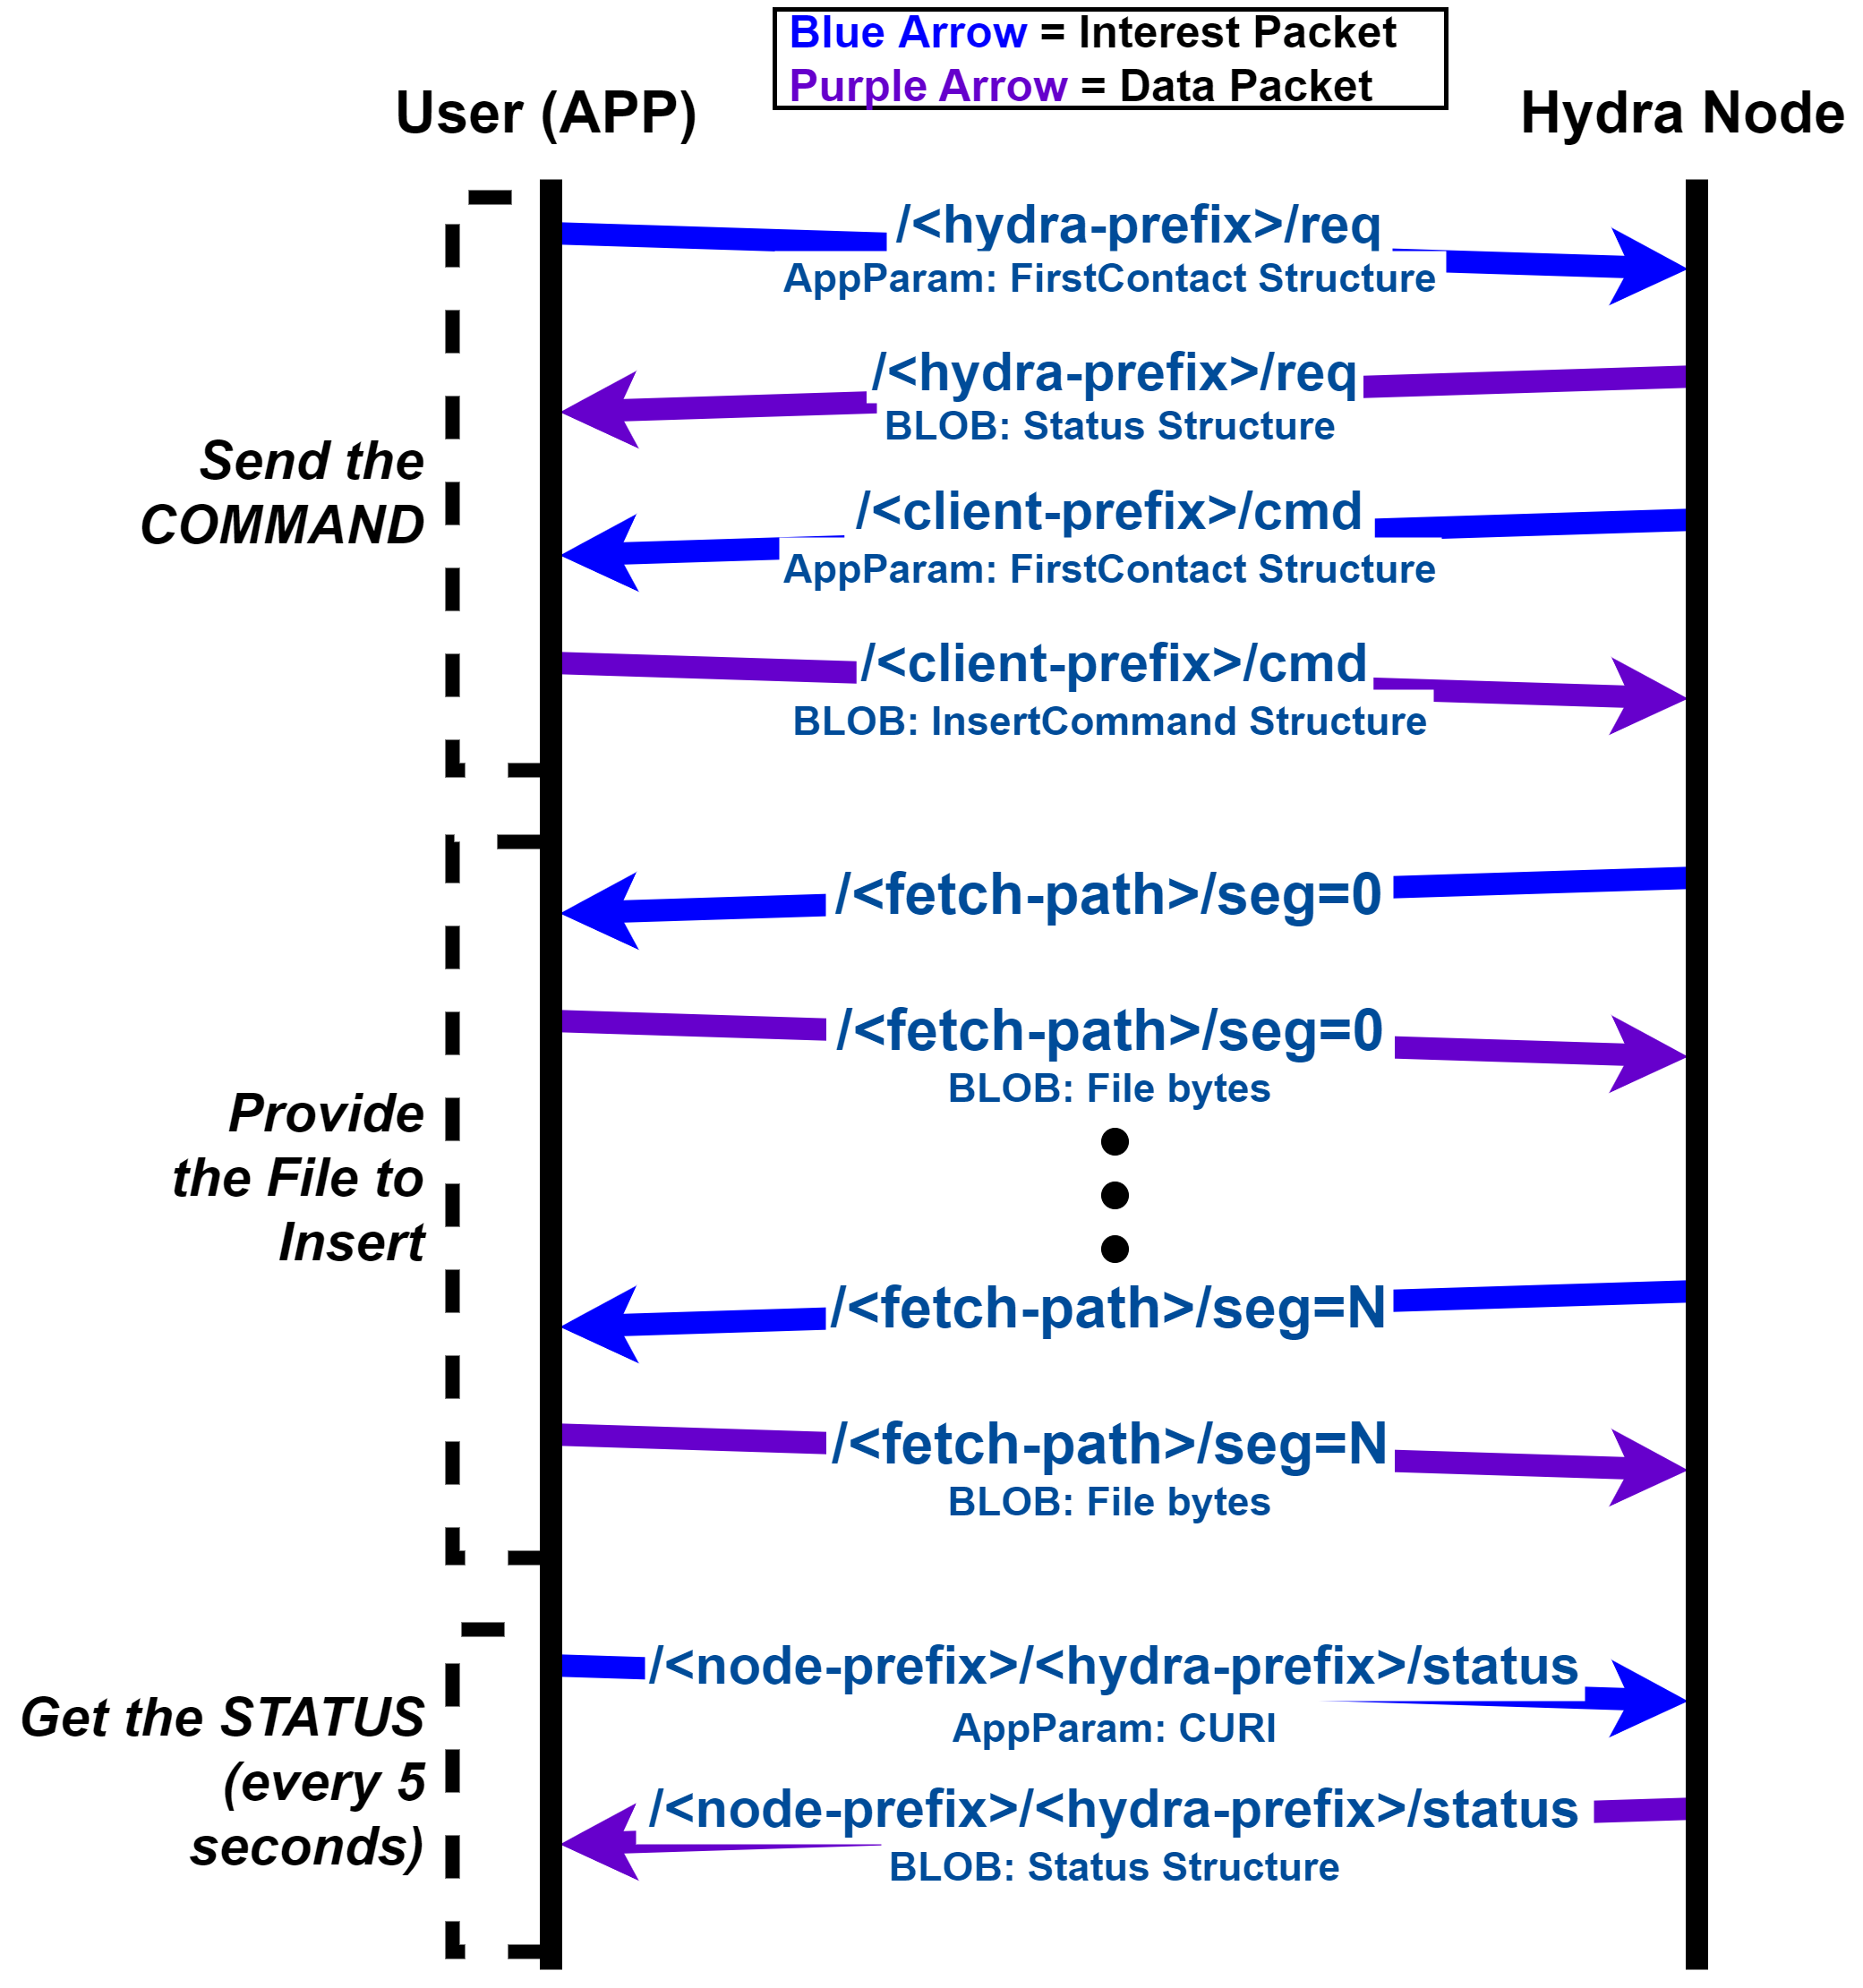
\includegraphics[width=\columnwidth]{visuals/insert-usr.png}
    \caption{NDN Interaction of A User and A Hydra Node During Data Insertion}
    \label{fig:insert-usr}
\end{figure}

The process of how a user will interact with a Hydra node via NDN is described in Figure~\ref{fig:insert-usr}. Any Hydra node can be contacted by the user for data insertion, and this interaction can be summarized as a PubSub-like interaction: it uses a notification Interest with a component /notify and data retrieval via /msg.
\todo[inline]{Define first contact structure and give and example}
\todo[inline]{user authentication is missing}
\xw{how to authenticate}
This interaction between user (A) and node (X) goes as follows:
\begin{enumerate}
    \item User (A) will send an Interest notification using the prefix /<hydra-prefix/insert, announcing that it has a command for any Hydra node to process.
    \item Upon hearing this, node (X) will send an Interest to fetch this command using user (A)'s prefix (stated in user (A)'s FirstContact structure found in the Interest notification's app parameters).
    \item Node (X) will begin to process this command; and because the command is an insertion, node (X) will begin to fetch file (F) using user (A)'s fetch path (found in the InsertCommand structure).
    \item Once file (F) is retrieved, node (X) will send a notification Interest stating that the command that user (a) sent has a updated status.
    \item User (A) can then fetch the status of the command using node (X)'s prefix (stated in node (X)'s FirstContact structure found in a previous interest).
\end{enumerate}

There are a few key points throughout this process.
\begin{enumerate}
    \item User (A) can fetch the status at any time as it has the necessary info; however if the command is not ready, node (X) will tell user (A) to wait. This is particularly useful in case node (X) goes offline. \todo[inline]{if X goes offline, how does it tell the user?}
    \item The switch from anycast to unicast is necessary to ensure a proper response as command information is not directly shared between Hydra nodes.
    \item Throughout the interaction, a command unique resource identifier (curi) is used. This allows Hydra nodes to process more than one command from a user and allows users to send more than one command.
    \todo[inline]{example of curi}
\end{enumerate}


\subsubsection{Module Interaction}
\begin{figure}[!ht]
    \centering
    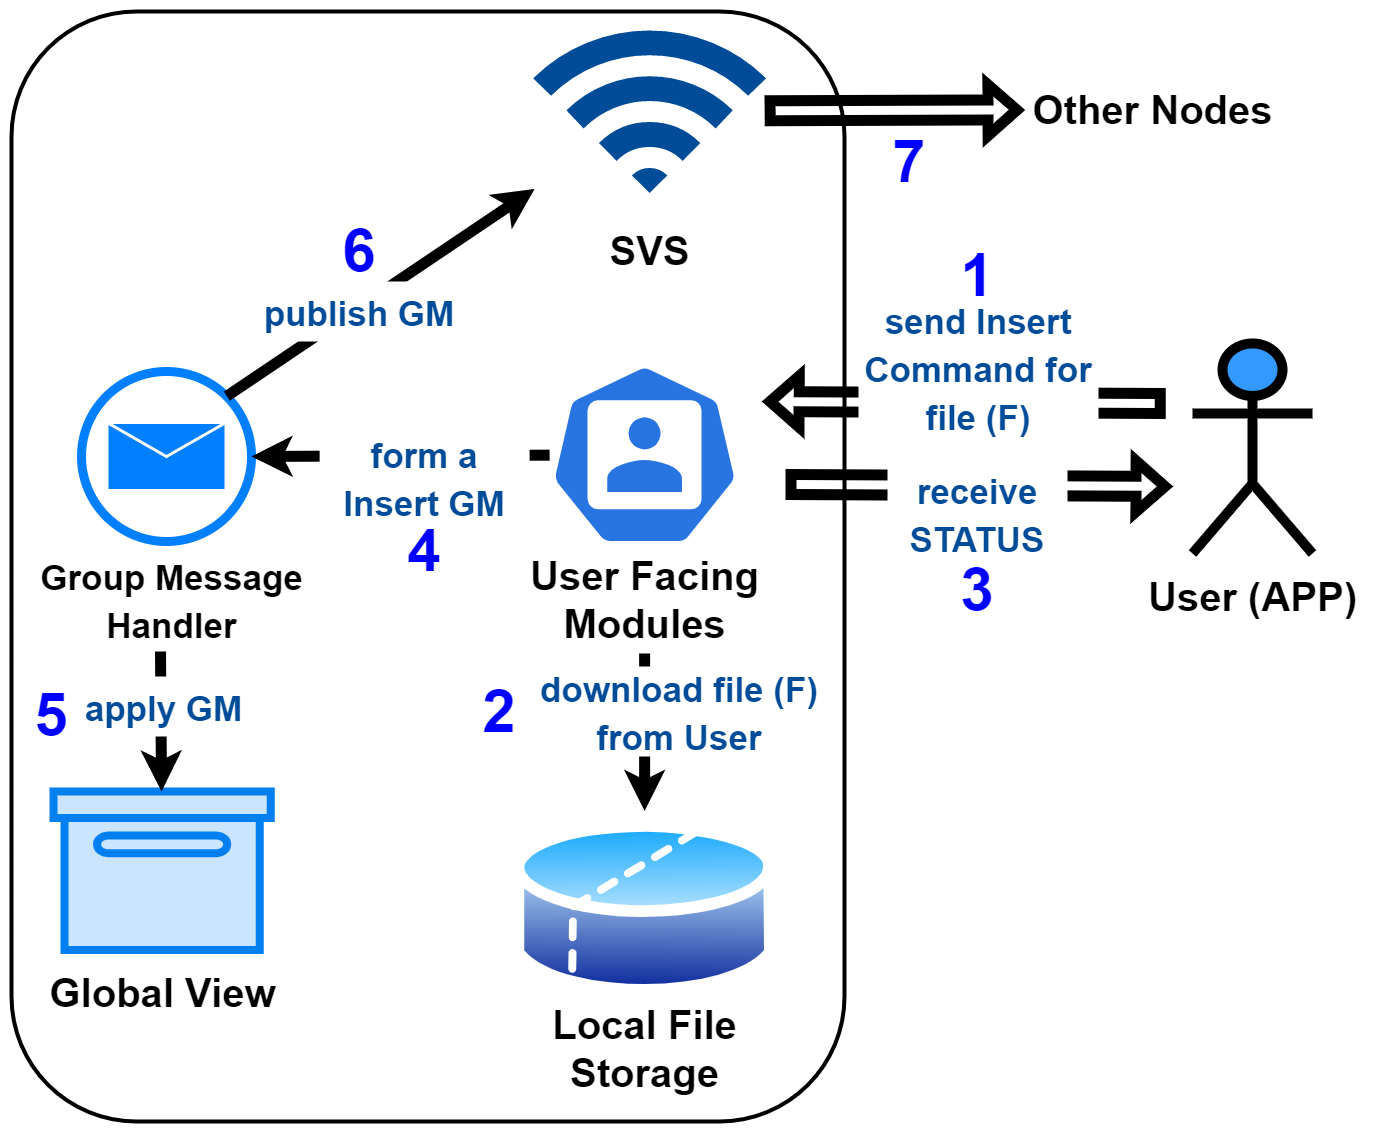
\includegraphics[width=\columnwidth]{visuals/insert-sys.png}
    \caption{Module Interaction to Fulfill a User's Insertion Command}
    \label{fig:insert-sys}
\end{figure}

The User-to-Node interaction leads to several interactions within Hydra.% node will act out the given command. 
Figure~\ref{fig:insert-sys} shows these interactions. When node (X) receives an Insertion command for file (F) from user (A):
\begin{enumerate}
    \item Node (X) properly authenticates the command, checks to see if the command can be executed, and then immediately starts fetching file (F) if the command satisfies all requirements.
    \item After storing file (F), node (X) updates the status for user (A) allowing user (A) to go offline.
    \item Node (X) then forms an Insert GM which includes all file metadata such as file name, size, etc. and states that node (X) will be storing this file.
    \item Node (X) applies this GM to its Global View.
    \item Node (X) publishes this GM using SVS, our distributed synchronization protocol.
\end{enumerate}

Every node will receive the Insert GM. When node (Y) receives the Insert GM sent by node (X) containing file (F)'s info, it performs the following operations:
\begin{enumerate}
    \item Node (Y) applies the GM to its Global View: file (F) information is added.
    \item Node (Y) sees that there is a replication need as file (F) does not meet the replication degree of 3 (stated in Hydra's base policy). For how replication is done, see Subsection~\ref{sec:data-replicate}
\end{enumerate}

\subsubsection{Data Structure Formats}
There are several structures that are used for the entire data insertion process. For the group message structures used in Module interaction, please refer back to Section~\ref{sec:group-messages}.

The structures used in User-to-Node interaction include the following:
\begin{enumerate}
    \item FirstContact: This includes the preferred name prefix that the sender wants to use for further interaction and a sender command unique resource identifier (curi) that the sender will use to refer to this interaction.
    \item InsertCommand: This include all necessary info that a Hydra node needs for a publication which includes a fetch path, file name, and other metainfo about the file.
    \item NotificationSpecification: This simply includes a command unique resource identifier (curi) of the receiver that the sender is referring to.
    \item CommandStatus: This just contains a Status code that can give simple feedback to the user. Theses codes are very simple and based on HTTP response status codes, please see Table \ref{tab:status-codes}. %\todo[inline]{define the status codes}
\end{enumerate}